\documentclass[11pt]{article}
\usepackage[margin=1in]{geometry}
\usepackage[utf8]{inputenc}
\IfFileExists{lmodern.sty}{\usepackage[T1]{fontenc}\usepackage{lmodern}}{}
\usepackage[expansion=false]{microtype}
\usepackage{amsmath,amssymb}
\usepackage{booktabs}
\usepackage{graphicx}
\usepackage{xcolor}
\usepackage{tikz}
\usetikzlibrary{arrows.meta,positioning}
\usepackage[numbers,sort&compress]{natbib}
\usepackage[colorlinks=true,linkcolor=blue!50!black,citecolor=blue!50!black,urlcolor=blue!50!black]{hyperref}
\usepackage{enumitem}
\setlist{itemsep=2pt,topsep=4pt}

\newcommand{\mb}{\textsc{MotionBench}}

\title{\mb{}: Goal-Referenced Evaluation of Robots, Code and People\\Where the Work Happens\\[0.4em]
\large Methodology and preliminary results --- a draft for public comment}
% Authors: fill in before submission. Student contributors who are minors may wish to
% appear by first name only or under the project name; check arXiv's authorship policy.
\author{The \mb{} contributors\\\small\url{https://motionbench.org} \quad \url{https://github.com/motionbenchmark/mb-core}}
\date{October 2026 \quad (draft v0.1)}

\begin{document}
\maketitle

\begin{abstract}
Is a team's autonomous code better than its own drivers? Does a robot vacuum cover a room
better than a person with a stick vacuum, or only faster? Questions like these come up
wherever robots do jobs, from student competitions to homes and warehouses, yet the
evaluations that could answer them are either private to a product or run in research labs
on standardized hardware. We describe \mb{}, an open benchmark that measures
\emph{whether a job gets done}, by any agent --- a person, team-written code, AI-written
code, a person with robot assistance, or a commercial robot --- in the space where the work
actually happens. Every task states a goal; every attempt is recorded as a trajectory
(from an ordinary phone video, printed fiducial tags or the robot's own log) and scored by
a single open, deterministic scorer as the share of that goal it achieved, with
uncertainty ranges, the worst run, and the level a randomly moving robot reaches.
Comparisons between people and machines are made only when both use the same means.
We describe the scoring model, the capture pipeline, the evaluation protocol, a game
simulator that runs unmodified VEX AIM Python code against simulated drivers with
explicit personalities, and a tool chain for multi-robot competition matches. We report
preliminary results that are clearly labelled: a tag-free phone capture of a household
robot vacuum, 120 motion-capture walks from an open dataset, simulated code-versus-driver
verdicts in which the best routine on a public layout loses its advantage on unseen
layouts, and a tracking benchmark for four-robot matches. Pilot studies with student teams
are planned; we publish the method now so that it can be criticised and improved before
those data exist.
\end{abstract}

\section{Introduction}

Robot competitions for students open every match with a period in which the robot runs
its own code, followed by a period of human driving. Teams argue, after nearly every match,
about which of the two is better. The argument has grown now that AI systems write robot code
too. It is a small instance of a general question --- \emph{how much of a job does this agent
get done?} --- that also applies to a household robot vacuum, a lawn mower, a warehouse
picker or a classroom arm.

Answering it fairly is harder than it looks. A match score mixes in the opponent, the field
and luck. A product page quotes its own best case. A raw number such as ``six targets in
eleven seconds'' means little without a statement of what the task was and what ``done''
means. And the strongest existing evaluations of robot behaviour are built for a different
purpose: research benchmarks fix the robot and the scene, and compare learned control
policies on standardized hardware~\cite{robodojo2026,libero2023,calvin2022,metaworld2019}.

\mb{} starts from the other end. It fixes the \emph{task and its goal}, and measures
whatever attempts it, on whatever hardware, where the attempt takes place. Its
contributions are:
\begin{enumerate}
  \item a \textbf{goal-referenced scoring model} that puts every kind of agent on one scale
    (share of the task's goal achieved), reports chance level instead of subtracting it,
    and allows a direct comparison with people only where the means are the same
    (Section~\ref{sec:scoring});
  \item an \textbf{outcome-only interface}: a run is a trajectory trace, so any agent can be
    scored without access to its code, including closed commercial products
    (Section~\ref{sec:traces});
  \item a \textbf{capture pipeline} that turns an ordinary phone video into a trace, with or
    without printed tags, and reports its own accuracy (Section~\ref{sec:capture});
  \item an \textbf{evaluation protocol} with public and unseen layouts, minimum run counts,
    tiers that separate simulated, field and verified results, and a dispute process
    (Section~\ref{sec:protocol});
  \item a \textbf{game simulator} that runs unmodified VEX AIM Python routines against
    simulated drivers with explicit traits, and returns a statistical verdict on whether the
    code beats people before it runs on a robot (Section~\ref{sec:games});
  \item tools for \textbf{multi-robot matches}: a match simulator, a renderer of
    broadcast-style video with ground truth, a per-robot report and a tracking benchmark
    (Section~\ref{sec:matches}).
\end{enumerate}
All code is released under Apache-2.0 and all task specifications and data under
CC~BY~4.0. Section~\ref{sec:prelim} reports preliminary results, most of them simulated
and labelled as such; Section~\ref{sec:plan} lists what the first pilots must establish.

\section{Related work}

\paragraph{Research benchmarks for robot policies.} Simulation suites such as
Meta-World~\cite{metaworld2019}, CALVIN~\cite{calvin2022} and LIBERO~\cite{libero2023}
evaluate learned manipulation policies on fixed robots and scenes; Habitat~\cite{habitat2019}
does the same for embodied navigation. SimplerEnv~\cite{simplerenv2024} studies how well
simulated evaluation predicts real-robot results. RoboDojo~\cite{robodojo2026} combines 42
simulated and 18 real-world tasks on standardized bimanual hardware, evaluates policies
through a shared policy-server interface, scores real trials by three blind evaluators with
partial credit, and checks submissions on hidden layouts. RoboArena~\cite{roboarena2025}
distributes real-world evaluation across institutions through pairwise comparisons.
These works share a design: the robot and setting are standardized, the learned policy is
the object of evaluation, and integration with the benchmark's software is required.
\mb{} differs on each point. The \emph{task} is standardized; the object of evaluation is the
whole agent (robot, software and, where present, its human operator); and the only
interface is the recorded outcome. We borrow from these benchmarks their emphasis on
explicit protocols, hidden layouts, repeatability measurements and separation of verified
from unverified results.

\paragraph{Human reference points.} Human-normalized scores were popularized by the Arcade
Learning Environment~\cite{ale2013,mnih2015}. \mb{}'s first specification used a similar
normalization to the median person on each task; we explain in Section~\ref{sec:scoring}
why we replaced it with a goal-referenced score.

\paragraph{Reporting under uncertainty.} Agarwal et al.~\cite{agarwal2021} show how point
estimates over few runs mislead, and recommend interval estimates and robust aggregates.
\mb{} reports percentile-bootstrap intervals~\cite{efron1979} on every mean, shares ranks
when intervals overlap, shows the worst run, and never aggregates across tasks.

\paragraph{Product performance standards.} Standards such as IEC~62929~\cite{iec62929}
specify laboratory test methods for household cleaning robots. \mb{} is complementary: it
measures robots in the spaces where they are used, from ordinary video, and places them on
the same scale as other ways of doing the same job.

\section{Design principles}
\begin{enumerate}[label=\textbf{P\arabic*}]
  \item \textbf{Goal first.} Every task states what ``done'' means, and every attempt is
    scored as the share of that goal it achieved.
  \item \textbf{Any agent.} People, team code, AI code, assisted people and commercial robots
    appear on the same board, labelled by who was in control.
  \item \textbf{Measured where robots work.} The benchmark comes to the robot: a phone, printed
    tags or the robot's log are enough. No special rig, and no access to the robot's code.
  \item \textbf{Re-scorable by anyone.} One open scorer, implemented once, gives the same
    report for the same trace every time; every published number can be recomputed.
  \item \textbf{Honest about uncertainty.} Ranges, the worst run, chance level, and labels
    that never let simulated results pass for real ones.
\end{enumerate}

\section{Tasks and goal-referenced scoring}\label{sec:scoring}

A \emph{task} specifies an arena (size, obstacles, zones), the robot's footprint, a time
budget, public layouts (start pose, waypoints or object positions) and a goal of one of
three kinds: \emph{waypoints} (reach each in order within a position and heading tolerance),
\emph{delivery} (each object rests in its target zone at the end) or \emph{coverage}
(share of free floor swept by a tool of given width). Table~\ref{tab:tasks} lists the
current tasks. They are game-neutral: they use competition hardware but never copy a
season's game.

\begin{table}[t]
\centering\small
\resizebox{\linewidth}{!}{%
\begin{tabular}{@{}llllll@{}}
\toprule
Task & Platform & Goal & Arena & Budget & People comparable \\
\midrule
MB-VEX-NAV@1.0 & VEX V5 & 6 waypoints, 5 cm / 5\textdegree & 3.66\,m square & 20\,s & yes \\
MB-VEX-PICK@1.0 & VEX V5 & deliver 6 objects & 3.66\,m square & 60\,s & yes \\
MB-AIM-NAV@0.1 & VEX AIM & 5 waypoints, 3 cm / 10\textdegree & 1.83 $\times$ 1.22\,m & 20\,s & yes \\
MB-AIM-SORT@0.1 & VEX AIM & sort 6 barrels by colour & 1.83 $\times$ 1.22\,m & 45\,s & yes \\
MB-COVER@0.1 & floor robots & cover free floor, 30\,cm tool & 4 $\times$ 3\,m & 180\,s & no \\
MB-FIELD-HALLWAY@0.1 & robot vacuum & cover visible floor & 1.3 $\times$ 3.0\,m & 137\,s & no \\
\bottomrule
\end{tabular}}
\caption{Current tasks (specification 0.2). ``People comparable'' marks tasks where a person
can do the same job with the same means, for example driving the same robot.}
\label{tab:tasks}
\end{table}

\paragraph{Goal score.} For a run with success $S$ in task units and maximum $S_{\max}$, the
goal score is $g = S / S_{\max} \in [0,1]$. For each agent, the board reports the mean goal
score over its runs with a 95\% percentile-bootstrap interval, the worst run, and the
\emph{completion rate}: the share of runs that achieved the whole goal.

\paragraph{Chance level.} Each board reports what a robot moving at random achieves, as a goal
score, beside the agents' scores. It is not subtracted: on coverage tasks a random walk
already covers about half of a room, and readers should see that, not have it hidden in a
transformation.

\paragraph{Why not normalize to people?} Our first specification scored every agent relative
to the median person on the task, following~\cite{mnih2015}. It failed in three ways. Where
people and machines use different means --- a robot vacuum against a person with a stick
vacuum --- normalization turned a difference in equipment into what looked like a
difference in skill. Many tasks have no like-for-like human run at all. And where most
people finish, the median sits near the maximum, so scores above the human level mostly
meant ``finished every time''. Specification 0.2 keeps the comparison with people as an
optional extra, reported only on tasks that declare \texttt{people\_comparable}:
$\mathrm{vs\_people} = (S - S_{\text{chance}})/(S_{\text{people median}} - S_{\text{chance}})$.

\paragraph{Secondary measures and the index.} Boards also report time to goal (over runs that
achieved it), path efficiency (shortest sensible path over path driven), consistency
($1 - \sigma/\mu$ of success) and safety ($1/(1+\text{violations})$, counting contacts with walls
and obstacles beyond a tolerance). A single index ranks agents within one task:
\[
\mathrm{MBI} = 0.50\,g + 0.20\,\mathrm{eff} + 0.15\,\mathrm{consistency} + 0.15\,\mathrm{safety},
\]
with every term in $[0,1]$. Scores are never averaged across tasks: a vacuum is never ranked
against a VEX robot.

\paragraph{Ranks.} Agents share a rank while their intervals overlap the interval of the
group's leader; a new rank starts only when an agent's upper bound falls below the leader's
lower bound.

\section{Traces and the scorer}\label{sec:traces}

A run is a directory (\texttt{.mbtrace}) with a manifest (task, layout, agent and its class,
capture method, tier, file hashes), poses sampled over time
(\texttt{t, x, y, $\theta$}), optional events (pickups, deliveries) and the final positions
of objects. The trace is the only interface between an agent and the benchmark. A team's
code, a person with a controller and a commercial robot all produce the same kind of file,
so none of them needs to be integrated with \mb{} software, and closed products can be
evaluated from video alone.

The scorer is implemented once, in Rust, and called from Python and the command line. It
checks the trace (hashes, monotonic time, sampling gaps), computes the run report and builds
the per-task board. A separate, self-contained explorer page re-counts waypoints, deliveries
and coverage from the raw poses in the browser and flags any run where its count and the
scorer's disagree, together with physical sanity checks (speed, leaving the arena, budget).

\section{Capture: from video to trace}\label{sec:capture}

\paragraph{With tags.} Four AprilTags~\cite{olson2011} in the arena corners and one on the robot
give a per-frame homography from image to floor; the robot tag gives position and heading.

\paragraph{Without tags.} Many interesting runs are filmed without preparation. For a fixed or
hand-held camera, frames are first aligned to the first frame (feature matching with a
similarity model), and the per-pixel median over the clip gives an empty-floor image. The
robot is the region that differs from it. The floor plane comes from four image points that
outline a rectangle on the floor~\cite{hartley2004}: its sides meet at a vanishing point that
fixes the floor's direction and tilt, and its far edge fixes the cross direction. What a
single view cannot give --- focal length and scale --- comes either from a measured width and
length, or from the robot itself, by searching for the focal length and camera height at
which a robot of known size matches its silhouettes. The robot's floor position is taken
half a robot behind the lowest point of its silhouette, smoothed, and heading follows the
direction of travel. Cells the camera cannot see are excluded from coverage and safety.

\paragraph{Accuracy.} The pipeline is tested on rendered video with known ground truth
(Table~\ref{tab:capture}); a real-world validation against tags is part of the first pilot.

\begin{table}[t]
\centering\small
\begin{tabular}{@{}lll@{}}
\toprule
Capture & Scale from & Position error (rendered test video) \\
\midrule
Printed tags & tag geometry & under 1 cm mean; robot found in 100\% of frames \\
No tags & measured floor width and length & about 2 cm median \\
No tags & robot size only & about 6 cm median \\
\bottomrule
\end{tabular}
\caption{Capture accuracy on synthetic video with ground truth (toolkit test suite).}
\label{tab:capture}
\end{table}

\section{Evaluation protocol}\label{sec:protocol}

\paragraph{Tiers.} Results are \emph{simulated} (S), \emph{field} (F: a real robot, captured and
submitted by its owner, reviewed by a person) or \emph{verified} (V). The three are never
mixed on one board without labels.

\paragraph{Runs.} An agent needs at least five runs on a task to be ranked (ten recommended).
Runs are consecutive attempts; every attempt in a session is reported.

\paragraph{Layouts.} Public layouts are published for practice. \emph{Unseen layouts} are drawn
from each task's layout rules with an unpublished seed, to separate agents that learned the
task from agents that learned a layout (Section~\ref{sec:prelim} shows why this matters).
Verified sessions use a layout drawn by \mb{} just before the session.

\paragraph{Verified runs.} A verified session requires: a layout sent at the start; one uncut
video from a fixed camera showing the whole arena, a code word sent at the start and every
run; a trace produced from tags or by a reviewer running the converter; all attempts
reported; the agent described (for code, the routine's version, shared privately on
request); and a second reviewer re-scoring at least one run from the raw video.

\paragraph{Repeatability and disputes.} The scorer is deterministic and every simulated run is
reproducible from its seed. Disputes are re-scored by a reviewer who did not score the
original, and every change to a published result is logged with the specification and
scorer versions and the date.

\paragraph{Minors and footage.} Many participants are students. Published results use
trajectories, not footage; videos showing people are not published without permission (for
minors, a parent's or guardian's).

\section{Games: code versus drivers in simulation}\label{sec:games}

\begin{figure}[t]
\centering
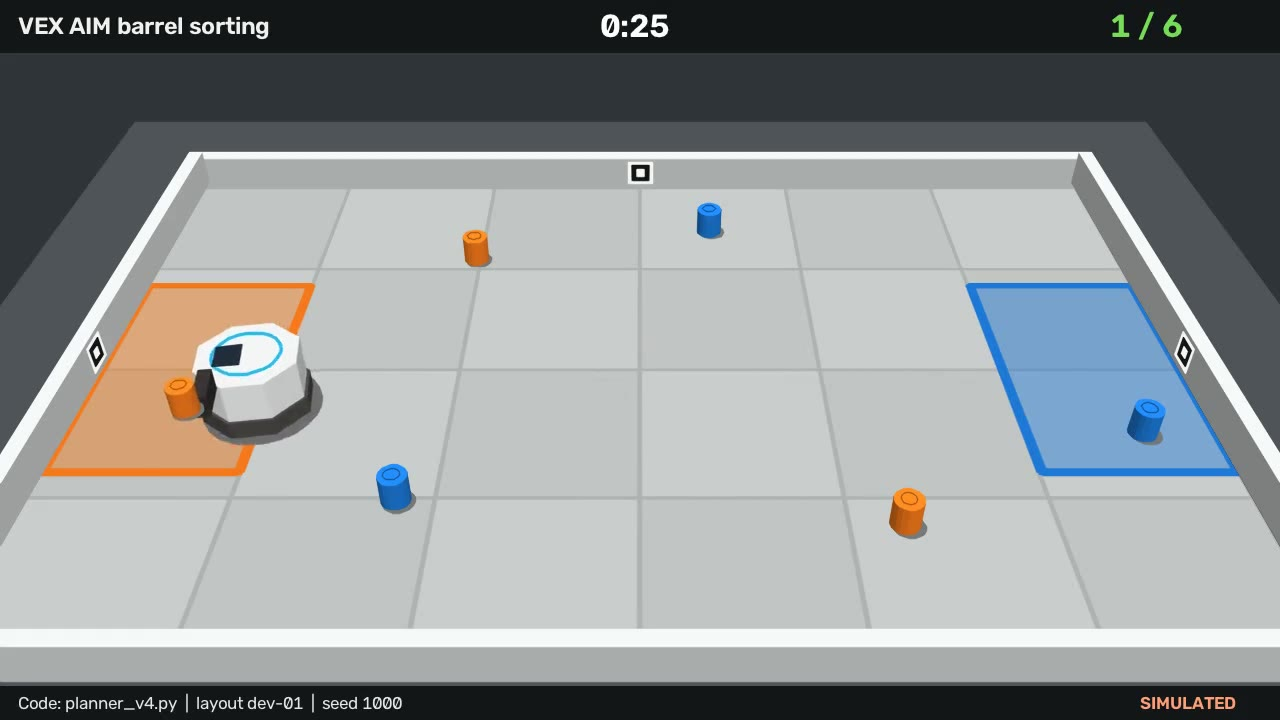
\includegraphics[width=0.49\linewidth]{figs/aim-sim.jpg}\hfill
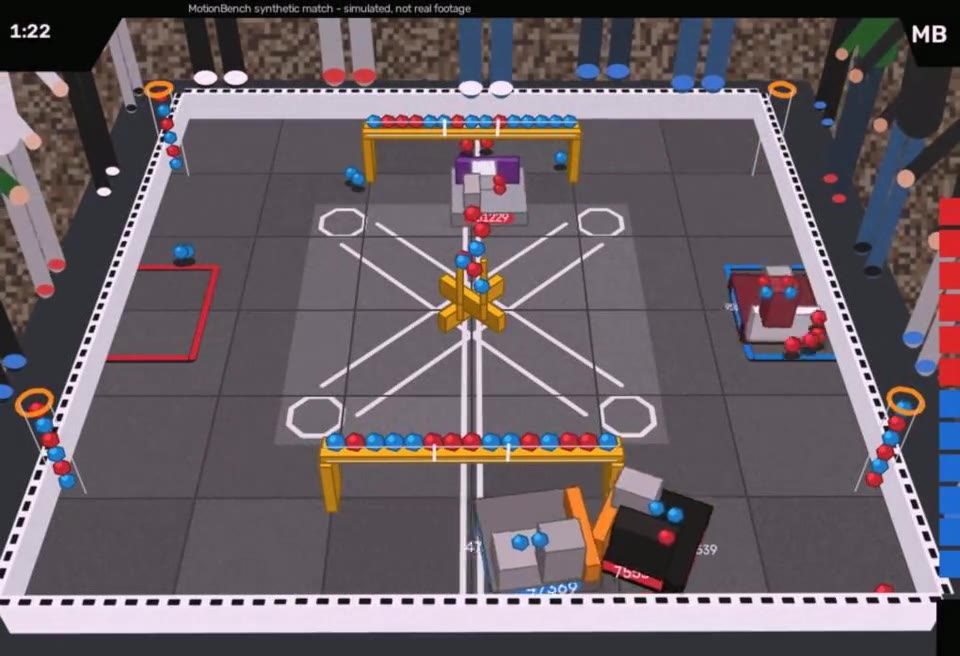
\includegraphics[width=0.49\linewidth]{figs/match-sim.jpg}
\caption{Simulated scenes, always labelled as such. Left: a VEX AIM routine sorting barrels in
the game simulator. Right: a four-robot VEX V5 match rendered from a camera position measured
from a real event broadcast.}
\label{fig:sims}
\end{figure}

A team that writes autonomous code wants to know, before testing on the robot, whether the
code will beat its drivers. \mb{} \emph{games} make that a repeatable experiment.

\paragraph{Games are defined once.} A game file records the field, scoring zones, wall-mounted
fiducials, object kinds, layouts, layout rules for generating new ones, match length and
scoring rules. For a team's own game it is written once from their code and a description of
the game, then validated; versions of the code are compared against the same definition. A
game may link to a \mb{} task with the same layouts, so that every simulated run is also
scored by the standard scorer --- and the two scores must agree.

\paragraph{Running code unchanged.} The first platform is VEX AIM, a small holonomic classroom
robot with a magnetic pick-up, a kicker and an AI camera. The simulator runs VEXcode AIM
Python files as written: the import header receives stand-ins for the robot, and every API
call (motion, inertial sensor, kicker, object sensing, camera detections of barrels and
AprilTags, waits) advances simulated time. Speeds follow the published API limits
(200\,mm/s, 150\textdegree/s). Each run draws its own imperfections --- wheel slip of a few
percent, sideways drift, turn overshoot, kick scatter, camera noise and missed detections ---
so routines that count wheel rotations accumulate error and routines that look at the field
can correct it. The match clock is enforced, busy loops consume time, and crashes stop the
robot and are reported.

\paragraph{Simulated drivers.} A driver is a controller policy with explicit traits: a reaction
time (the driver acts on a delayed view of the field, partly anticipating the robot's motion),
the share of full speed used, steering shake, placement precision, decision quality (choice of
the next object), mistake rate and hesitation. Six named characters span a classroom, from a
first-week driver to a team's best; a simulated class of twenty drivers with traits drawn
around them defines the \emph{typical student}, the median of the class. These are models
chosen to be plausible, not measurements of anyone.

\paragraph{Verdict.} Each routine runs 20 times and each character 12 times; the typical student
runs as often as the code. Every comparison is the difference of mean points with a 95\%
bootstrap interval, reported as \emph{better}, \emph{worse} or \emph{can't tell}. Verdicts are
given on the public layout and on unseen generated layouts.

\section{Multi-robot matches}\label{sec:matches}

Competition matches have four robots, two alliances and no tags. Scoring individual robots in
a match first requires knowing where each was. From a screen recording of an event broadcast
we kept only measurements: after a short intro, the broadcast uses a fixed overhead camera,
which the four field corners alone place at about 3.7\,m above the floor, tilted about
44\textdegree{} down (focal length $\approx$1139\,px at $1020\times696$). The footage itself is
not published.

The tool chain contains a seeded 2-versus-2 match simulator (autonomous and driver periods,
pushing, objects carried and delivered, parking), a renderer that films simulated matches
from the measured camera with people, an overlay and compression noise, and writes per-frame
ground truth; a per-robot report (distance, speed, idle time, time in each half, contacts,
split by period) that works equally on simulated and tracked matches; and a tracking benchmark
reporting recall, precision, position error, identity switches, MOTA~\cite{bernardin2008} and
IDF1~\cite{ristani2016}. A baseline tracker uses an occupancy map: for every floor position,
the camera model gives the image box a robot standing there would fill, and robots are where
that box is full of foreground and its surroundings are not.

\section{Preliminary results}\label{sec:prelim}

All results in this section are either simulated or single real captures. They test the
method; they are not measurements of any product, team or person.

\paragraph{A robot vacuum from one phone video.} A household robot vacuum was filmed for 137\,s
with a hand-held phone at the end of a hallway, without tags. Scale came from the robot's size;
floor the camera could not see was excluded. The vacuum covered 85\% of the 3.24\,m$^2$ of
visible floor with a 30\,cm cleaning width (51\% of it more than once), driving 18.6\,m. Most
of the missed area is a thin strip along the walls that a side brush cleans and our model does
not credit --- a limitation the coverage goal now addresses with an optional edge-reach
parameter.

\paragraph{People as agents.} We scored 120 motion-capture walks along one route
(about 7\,m) from the open THÖR-MAGNI dataset~\cite{thormagni2024}. All 120 reached the goal
(median 6.8\,s), so success alone could not separate the walkers; time, path efficiency and
consistency did. With a 60\,s budget, a random walk reached the goal in 40\% of runs, showing
that time budgets should follow typical completion times. The same saturation appears in our
synthetic VEX navigation board, where 7 of 19 agents achieve the whole goal on every run.

\paragraph{Code versus drivers, and unseen layouts.} Four sample routines for the AIM sorting
game (Figure~\ref{fig:verdict}) range from a fixed plan without sensors to a planner that
chooses an efficient order and uses the camera only for the final approach. On the public
layout, the planner averages 4.0 of 6 points against 2.8 for the typical simulated student, a
difference of $+1.3$ (95\% interval $+1.1$ to $+1.6$), and is level with the two best drivers.
On ten unseen layouts it drops to 2.8, level with the typical student ($-0.1$, interval
$-0.55$ to $+0.3$), because its plan encodes where the barrels are on the public layout. The
routine that searches for barrels with the camera barely changes (2.45 to 2.40). The
simulated drivers are unaffected by the change of layout. A verdict on public layouts alone
would have promoted the wrong routine. The simulation also showed that, at the AIM robot's top
speed, no agent sorts all six barrels in 45\,s; the best runs score 4 or 5.

\begin{figure}[t]
\centering
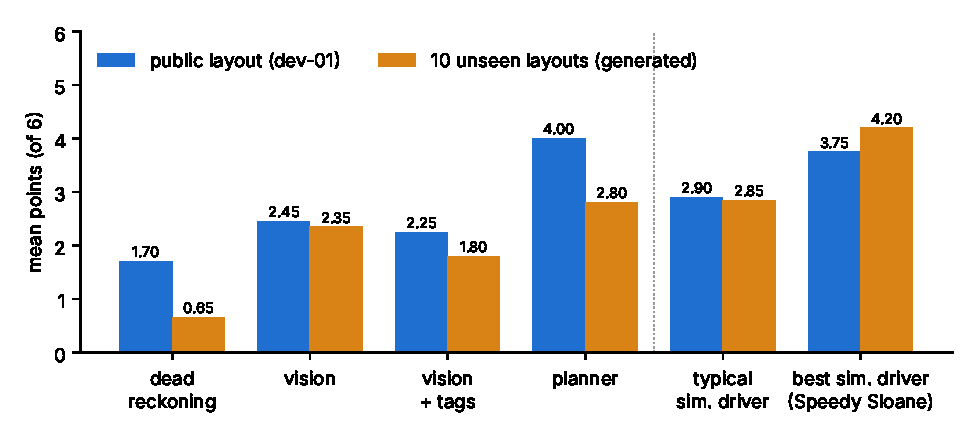
\includegraphics[width=\linewidth]{figs/verdict-unseen.pdf}
\caption{Simulated AIM sorting: mean points on the public layout and on ten unseen layouts, for
four routines, the typical simulated student and the best simulated driver (20 runs per
routine, 12 per driver).}
\label{fig:verdict}
\end{figure}

\paragraph{Tracking four robots.} On three simulated matches rendered from the measured camera,
the baseline tracker finds 90--97\% of robot positions with a median error of 7--9\,cm, but
keeps identities poorly: 25--44 identity switches per two-minute match and IDF1 of 48--66\%,
mostly when robots push each other (Table~\ref{tab:match}). On one minute of the real broadcast
it kept a track on all four robots, with one identity change and the correct alliance for four
of five tracks; without ground truth for the real clip, this describes behaviour, not accuracy.

\begin{table}[t]
\centering\small
\begin{tabular}{@{}lccccccc@{}}
\toprule
Match & Recall & Precision & Median err. & 90\% err. & ID switches & IDF1 & Alliance \\
\midrule
m0001 & 97.1\% & 98.6\% & 8.0\,cm & 17.7\,cm & 25 & 65.1\% & 68.4\% \\
m0002 & 89.5\% & 95.8\% & 8.9\,cm & 19.1\,cm & 33 & 65.6\% & 90.6\% \\
m0003 & 90.4\% & 94.3\% & 7.0\,cm & 15.8\,cm & 43 & 48.3\% & 61.5\% \\
\bottomrule
\end{tabular}
\caption{Baseline tracker on simulated four-robot matches (10\,fps, gate 0.45\,m).}
\label{tab:match}
\end{table}

\section{What the first pilots must establish}\label{sec:plan}

\begin{enumerate}
  \item \textbf{Drivers versus their own code} on MB-VEX-NAV and MB-VEX-PICK with student teams:
    at least ten runs per agent, public and unseen layouts, tags and tag-free capture of the same runs.
  \item \textbf{Capture validity on real video}: tag-free position error measured against tags on
    the same runs, across rooms, lighting and camera placements.
  \item \textbf{Paired simulation and reality}: the same AIM routines run in the game simulator and
    on a real robot on the same layouts, reporting the gap per routine.
  \item \textbf{Calibrated drivers}: driver traits fitted to filmed runs of real students, and the
    verdict re-checked with calibrated drivers.
  \item \textbf{Repeatability}: repeated sessions with the same robot and agent, reporting spread.
  \item \textbf{Hand-labelled match frames} from footage used with permission, to measure tracking
    accuracy on real matches.
\end{enumerate}

\section{Limitations}

Most current results are simulated, and simulation encodes our assumptions: robot size,
accelerations, camera field of view, friction and every driver trait are estimates. The synthetic
VEX AIM boards published with specification 0.2 contain simulated agents faster than the AIM
robot's published top speed; they are being regenerated with the limit used by the game simulator.
Tag-free capture depends on a visible floor rectangle and a fixed camera position after
stabilization. Coverage tasks reward a model of cleaning, not cleaning itself. The match tracker
does not yet keep identities reliably. Goal scores depend on how a task's goal and budget are set,
which is why tasks, layouts and protocol are published and changed only through public RFCs.

\section{Conclusion}

\mb{} measures whether a job gets done, by any agent, where the work happens, with an open scorer
anyone can rerun. We publish the method, the tools and the preliminary results before the pilots,
so that they can be criticised and improved first. Comments, tasks and runs are welcome at
\url{https://motionbench.org} and in the project's GitHub discussions.

\paragraph{Acknowledgements.} We thank the THÖR-MAGNI authors for releasing their data. Parts of
the software and of this manuscript were drafted with the help of an AI assistant; the authors
reviewed, tested and take responsibility for all of it.

\bibliographystyle{plainnat}
\bibliography{refs}

\appendix
\section{Reproducing the results}
\small
\begin{verbatim}
pip install "motionbench[tracker]"                    # or build from source
motionbench synth --out data/synthetic-v0.1           # synthetic boards
motionbench aggregate data/synthetic-v0.1 -o board.json
R=games/aim-sort/routines
motionbench game verdict games/aim-sort --layout dev-01 \
  --code $R/deadreckon_v1.py --code $R/vision_v2.py \
  --code $R/vision_tags_v3.py --code $R/planner_v4.py
motionbench match synth -o data/match-sim-v0.1 --seeds 1-5
motionbench match render data/match-sim-v0.1/m0001 -o m0001.mp4 --fps 10 --seed 1
motionbench match track m0001.mp4 -o tracks.csv
motionbench match eval data/match-sim-v0.1/m0001 tracks.csv
\end{verbatim}
\end{document}
